\documentclass{article}

\usepackage{geometry}

\usepackage{fancyhdr}
\lhead{Szymon Szulc\\z1193274}
\rhead{\today\\Programowanie współbieżne}
\thispagestyle{fancy}

\usepackage{polski}
\usepackage{amssymb}
\usepackage{amsthm}
\usepackage{amsmath}
\usepackage{xcolor}
\usepackage{multicol}
\usepackage{graphicx}

\usepackage[utf8]{inputenc}
\setlength{\parindent}{0pt} 
\setlength{\headheight}{24pt} 

\newtheorem*{lemma}{Lemma}

\begin{document}

\begin{center}
    {\LARGE \textbf{Sortowanie bitoniczne}} \\[1em]
\end{center}

\section*{Opis algorytmu}
Sortowanie bitoniczne nie było żadnym z zadań na kursach ASD. Urzekło mnie ono swoim wzorem wywołań, naprzemiennie obserwujemy wywołania \texttt{bitSortUp} i \texttt{bitSortDown}. Dodatkowo należy do klasy algorytmów \textit{niepomnych} - każde wywołanie dotyka tych samych komórek pamięci. Łącząc \textit{niepomność} z brakiem konfliktów odczytu i zapisu otrzymujemy, wydaje się, prawie idealny algorytm sortujący do zrównoleglenia. \\ 
Spójrzmy na sam algorytm:
\begin{multicols}{2}
\begin{verbatim}
void bit_merge(
  long long* ar,
  size_t left,
  size_t right,
  size_t n,
  int dir)
{
  if (n == 1) return;
  size_t mid = (left + right) / 2;
  size_t half = n / 2;
  for (size_t i = 0; i < half; ++i)
    bitonic_swap(
        ar,
        left + i,
        mid + i,
        dir);
  bit_merge(ar, left, mid, n/2, dir);
  bit_merge(ar, mid, right, n/2, dir);
}
\end{verbatim}
\columnbreak
\begin{verbatim}
void bit_sort(
  long long* ar,
  size_t left,
  size_t right,
  size_t n,
  int dir)
{
  if (n == 1) return;
  size_t mid = (left + right) / 2;
  bit_sort(ar, left, mid, n/2, ASC);
  bit_sort(ar, mid, right, n/2, DESC);
  bit_merge(ar, left, right, n, dir);
}
\end{verbatim}
\end{multicols}
Sortowanie bitoniczne ma jedną wadę, długość tablicy wejściowej musi być postaci $2^k$. Łatwo można sobie z tym poradzić dopełniając tablicę do najbliższej potęgi $2$ wartością $\infty$ (na przykład \texttt{LONG LONG MAX}), a potem ucinając nadmiarowy koniec posortowanej zmodyfikowanej tablicy.
\subsection*{Złożoności}
Klasyczny algorytm w wersji $1$ wątkowej ma złożoność czasową: $\mathcal{O}(n\ln^2(n))$, co otrzymujemy wprost z \textit{Twierdzania o rekursji uniwersalnej}. \\ 
Złożoność pamięciowa: $\mathcal{O}(\ln^2(n))$ przez rekursję, samo sortowanie następuje \textit{w miejscu}.

\newpage 

\subsection*{Model PRAM}
Jeśli zrównoleglimy pętlę \texttt{for} i wszystkie podwywołania w rekursji to otrzymamy: \\
$T(n) = \mathcal{O}(\ln^2(n))$ \\ 
$W(n) = \mathcal{O}(n\ln^2(n))$ \\
Brak konfliktów odczytu i zapisu, więc jesteśmy w klasie \textbf{EREW}.

\section*{Optymalizacje}
Zawsze dobrym pomysłem jest uciąć rekursję w porę, więc od pewnego rozmiaru podzadania zamiast zagłębiać się rekurencyjnie wywołuję \texttt{insertionSort}.

\begin{figure}[htp]
    \centering
    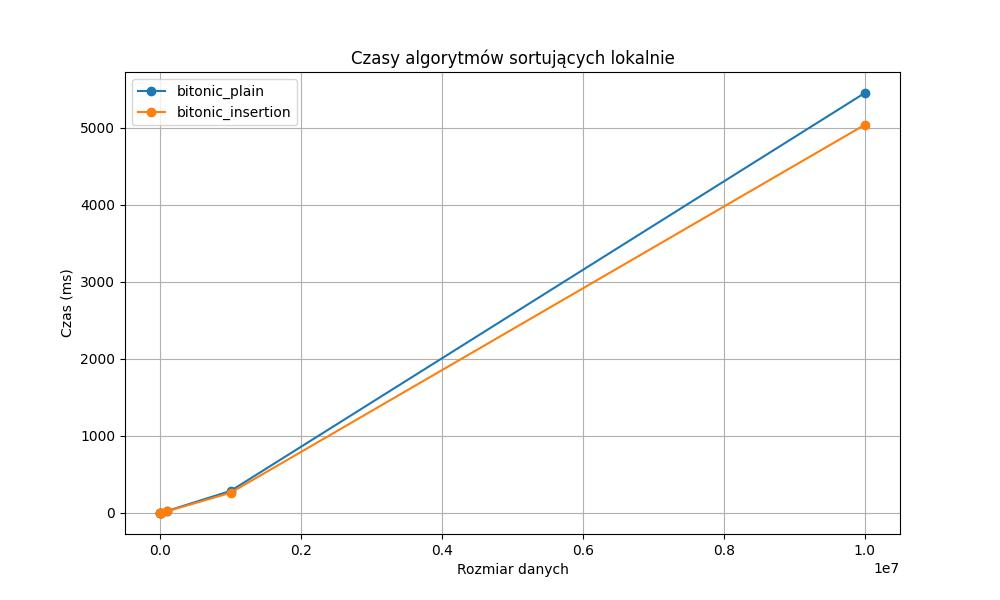
\includegraphics[width=0.8\textwidth]{czasy_lokalne_opt.jpg}
    \caption{klasyczny bitonicSort vs bitonicSortWithInsertion}
\end{figure}
Nie poprawiło to wydajności, tak jakbym się spodziewał. Lepsze wyniki osiągnelibyśmy zastępując \texttt{bitMerge} scalaniem podobnym jak w \texttt{mergeSort}, ale wtedy algorytm wykorzystywałby dodatkową pamięć, czego nie chciałem.

\newpage

\section*{OpenMP}
Bibliotekę \textbf{OpenMP} wykorzystałem do zrównoleglenia rekurencyjnych podzadań \texttt{bitSort}. Utworzyłem pojedynczą grupę wątków nad korzeniem rekursji i pozwoliłem bibliotece zarządzać wątkami w podzadaniach. Przed \texttt{bitMerge} zsynchronizowałem wątki. Próba zrównoleglenia również pętli \texttt{for} w \texttt{bitMerge} zakończyła się niepowodzeniem, wątki zaczynały walczyć o zasoby i czas wykonania się diametralnie wydłużał.
\begin{multicols}{2}
\begin{verbatim}
...
#pragma omp parallel
 {
   #pragma omp single 
   {
     bit_sort_omp(...);
   }
 }
...
\end{verbatim}
\columnbreak
\begin{verbatim}
...
#pragma omp task
  bit_sort_omp(ar, left, mid, n/2, ASC);
#pragma omp task
  bit_sort_omp(ar, mid, right, n/2, DESC);
#pragma omp taskwait
  bit_merge_omp(ar, left, right, n, dir);
...
\end{verbatim}
\end{multicols}

\section*{Wątki systemowe}
Tutaj zasada zrównoleglenia jest bardzo podobna. Ustaliłem granicę, powyżej której funkcja będzie wielowątkowa. Poniżej tego poziomu nakład zarządzania wątkami może przekroczyć czas działania wersji $1$ wątkowej. Załóżmy, że dane są odpowiednio duże. 
\begin{enumerate}
    \item Najpierw ustalona przeze mnie liczba wątków podzieli się tablicą z danymi. Każdy wątek będzie odpowiedzialny za swój blok.
    \item Wątki sortują bloki wywołując \texttt{bitSort} na bloku.
    \item Synchronizacja.
    \item Dwukrotnie maleje liczba wątków, dwukrotnie zwiększa się rozmiar bloku. Jesteśmy teraz w momencie, kiedy klasyczny \texttt{bitSort} wchodzi do góry od liści wykonując tylko \texttt{bitMerge}.
    \item Wątki scalają bloki wywołując \texttt{bitMerge}.
    \item Synchronizacja.
    \item Zmniejszenie liczby wątków, zwiększenie rozmiarów bloków.
    \item ... aż rozmiar bloku, będzie równy rozmiarowi tablicy wejściowej.
\end{enumerate}
Z moich obliczeń wynika, że: \\
$T(n) = \mathcal{O}(n\ln(n))$ \\
$W(n) = \mathcal{O}(n\ln^2(n))$ bez zmian

\newpage

\section*{Pomiary czasowe}
Lokalne pomiary przeprowadziłem na procesorze z $16$ rdzeniami. Raz \texttt{scheduler} tak ułożył wątki, że moje sortowanie bitoniczne na wątkach systemowych wyprzedziło \texttt{sort} z \texttt{STL} o $300ms$. To się już nigdy nie powtórzyło. 
\begin{figure}[htp]
    \centering
    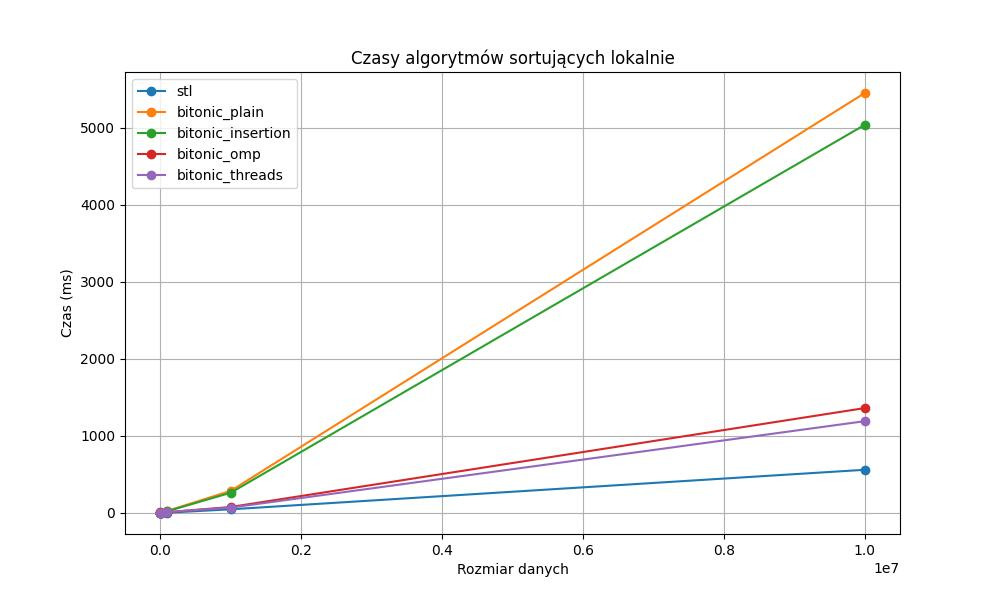
\includegraphics[width=0.7\textwidth]{czasy_lokalne.jpg}
    \caption{Pomiary lokalne}
    \centering
    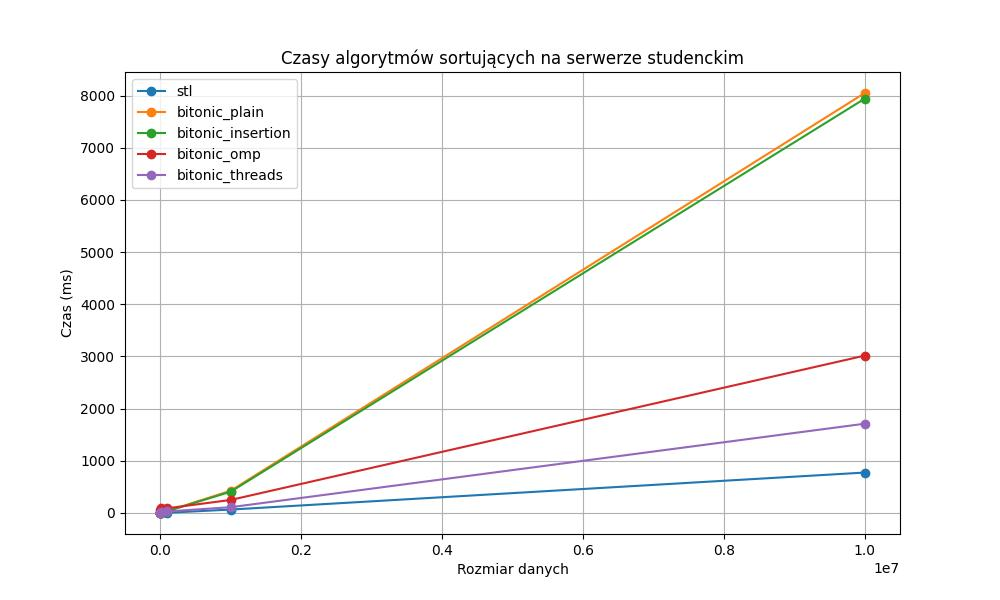
\includegraphics[width=0.7\textwidth]{czasy_student.jpg}
    \caption{Pomiary na serwerze student}
\end{figure}
\newpage 

\begin{figure}[htp]
    \centering
    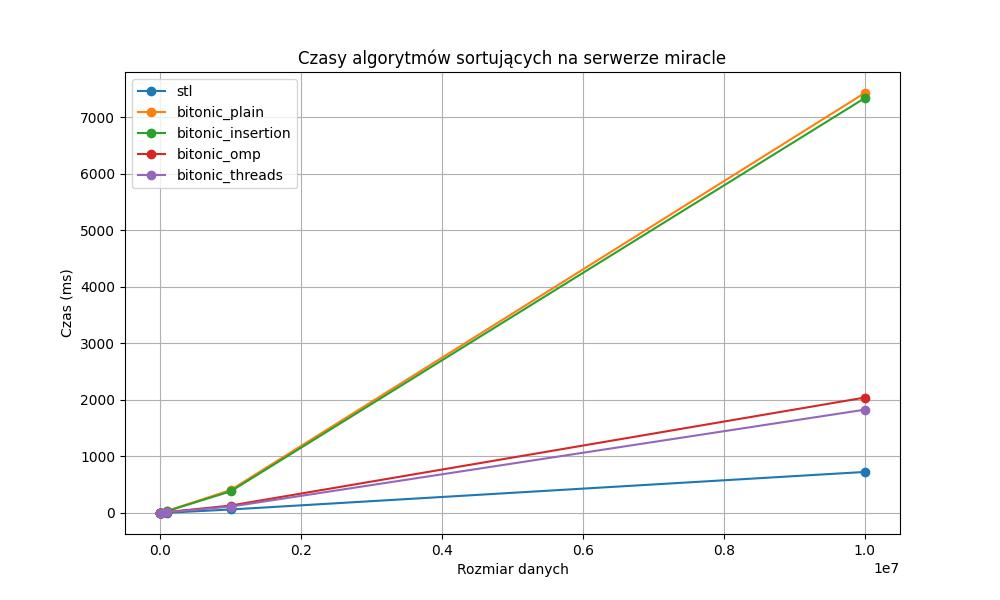
\includegraphics[width=0.7\textwidth]{czasy_miracle.jpg}
    \caption{Pomiary na serwerze miracle}
\end{figure}


Jak widać na powyższych wykresach:
\begin{enumerate}
\item Nie udało mi się pokonać \texttt{sorta} z \texttt{STL}.
\item \textbf{OpenMP} działa zauważalnie gorzej na studencie.
\item Sukcesem jest, że lepiej zarządzam wątkami niż robi to biblioteka \textbf{OpenMP}
\end{enumerate}

\section*{Podsumowanie}
Mojej implementacji jest daleko od idealnej sieci sortującej. Wyniki pokazują również, jak bardzo dopracowany jest \texttt{sort} z \texttt{STL}. Być może na \textbf{CUDA} udałoby się pokonać \texttt{sort} z \texttt{STL}.

\newpage

\section*{CUDA (aktualizacja po czasie)}
W końcu udało mi się zebrać do implementacji sortowania bitonicznego na CUDA i wyniki są bardzo zadowalające. \texttt{sort} z STL został pokonany ;).

\begin{figure}[htp]
    \centering
    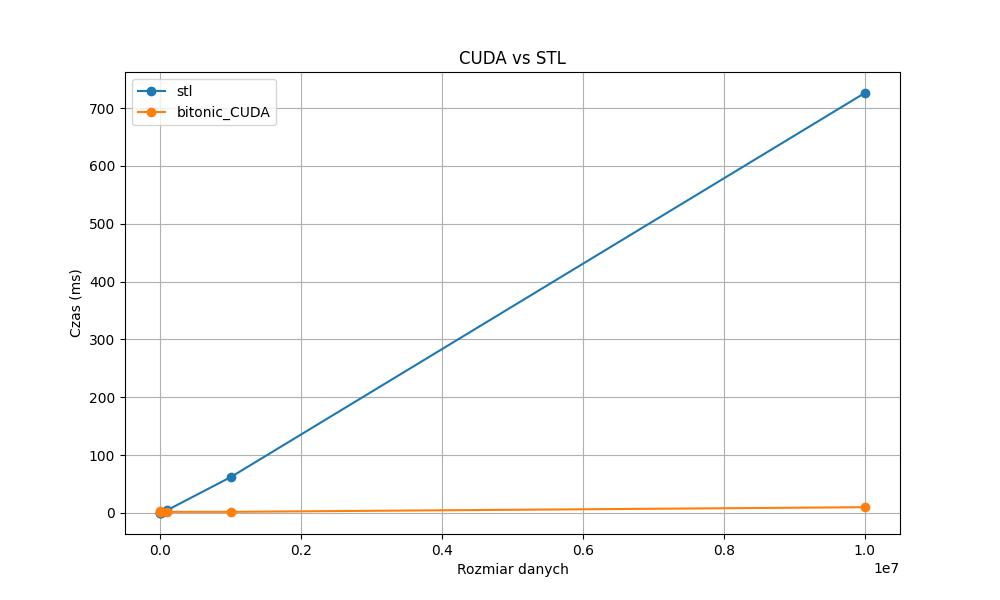
\includegraphics[width=0.7\textwidth]{stlVsCUDA.jpg}
    \caption{STL vs CUDA}
\end{figure}

Kilka słów o implementacji:
\begin{enumerate}
    \item Całość opiera się o 2 pętle \texttt{for}. Jedna przebiega po rozmiarze podzadania w sortowaniu bitonicznym, a druga udaje mergowanie.
    \item Równoległość osiągnięta z pomocą biblioteki \texttt{moderngpu} (powodem jest tylko i wyłącznie moja wygoda, żeby samemu nie pisać kerneli). 
\end{enumerate}

\end{document}
